\section{Additional numerical investigation}
\label{2406:sec:app:hyperparams}
In this appendix, we provide additional details on the numerical implementations presented in the main text, along with further explorations. The code to reproduce representative figures is available in \href{https://github.com/IdePHICS/batch-size-time-complexity-tradeoffs}{our GitHub repository}.

\subsection{Cold start for multi-index models} \label{2406:app:multiindex_model}
The theoretical considerations for weak recovery under cold starts presented in Theorems~\ref{2406:thm:main:sgd_weak_recovery}\&\ref{2406:thm:main:no_yhat_weak_recovery} are proven rigorously just for one-hidden neuron network learning single-index targets (\(p=k=1\)); this section aims to provide arguments to generalize this to the multi-index case. 

Note that for single-index models the initial saddle is the only critical point where the algorithm can get stuck during the dynamics, while this is not true in general for multi-index settings. Indeed, after having weakly recovered a subspace of the span of the target weights, the learning dynamics can encounter another saddle of the loss function; this behavior is known as saddle-to-saddle dynamics \cite{jacot2022saddle}. In this manuscript, we focus on escaping from the saddle at initialization, leaving further explorations of the dynamics to future work. We follow 
\cite{abbe2023sgd,dandi2023how} where the authors generalize the concept of Information Exponent (defined in.~\eqref{2406:def:main:information_exponent}) to the multi-index setting (See Definition $1$ of \cite{abbe2023sgd} and Definition $3$ of \cite{dandi2023how}), let us call this quantity the \textit{Leap Index} of the target.
We expect that, as long as the dynamics around the saddle at initialization is analyzed, one can substitute the Information Exponent ($\ell$) of the teacher in the single-index phase diagram in Fig.~\ref{2406:fig:cold_start_pd} with the Leap Index of the target. We explore the Time~/~Complexity tradeoffs in Figure~\ref{2406:fig:app:multiindex} for a fixed teacher function with Leap Index equal to $3$: we observe a relevant decrease in the iterations needed to weakly recover the target subspace as the batch size is increased.  

\begin{figure}
    \centering
    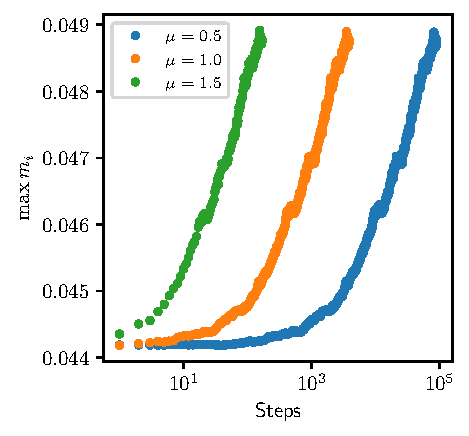
\includegraphics[width=.5\textwidth]{figs/multiindex_mu}
    \caption{\textbf{{Multi-index large-batch benefits:}} Comparison between the performance of plain SGD learning multi-index model, for different values of \(\mu\). The target is \(h^\star(z_1,z_2,z_3)=\tanh{(z_1z_2z_3)}\), while the student is a wide 2-layer network \(f(\vec{x})=\frac1p\sum^p_{i=1}\tanh(\vec{w}_i\cdot\vec{x})\) (hence \(\ell=3,p=30, k=3, d=512\)). Using a larger batch speeds up the weak-correlation time even when the target is multi-index, and it is learned with a non-matching architecture.
    }
\label{2406:fig:app:multiindex}
\end{figure}


% \textcolor{blue}{\textbf{LP: To change} the behavior of the dynamics \emph{at initialization} does not change from the single-index to multi-index case. The model will initially learn one direction in the target subspace, effectively behaving like a single index model.  This intuition is numerically proved by the experiment in Figure~\ref{2406:fig:app:multiindex}: Correlation Loss can learn while plain Projected SGD, not only cannot escape the initial saddle but jumps to higher test error saddles. Similar results can be obtained for different choices of activation functions with \(\ell\ge3\). }

\subsection{Behavior of \emph{Spherical SGD}}
In many theoretical work \cite{arous2021online,abbe2023sgd}, % TODO cite more
the algorithm used during training uses the \emph{spherical gradient} instead of the simple one. The update rule used instead of Equation~\eqref{2406:eq:gd_update_weight} is
\begin{align}
    \vec w_{j,t+1} =  \frac{\vec{w}_{j,t} - \gamma \left(I_d-\vec{w}_{j,t}\vec{w}_{j,t}^\top\right)\nabla_{\vec w_{j,t}}\ell_t}{\norm{\vec{w}_{j,t} - \gamma \left(I_d-\vec{w}_{j,t}\vec{w}_{j,t}^\top\right)\nabla_{\vec w_{j,t}}\ell_t}} \qquad \forall t \in [T],   \forall j \in [p]
    \label{2406:eq:app:gd_update_weights}
\end{align}
In practice, only the gradient component orthogonal to the weights is taken into account. This algorithm is particularly convenient for theoretical analysis because it is easier to find a lower bound for the evolution of \(m_t\), since it is always true that 
\[
    \norm{\vec{w}_{j,t} - \gamma \left(I_d-\vec{w}_{j,t}\vec{w}_{j,t}^\top\right)\nabla_{\vec w_{j,t}}\ell_t} \ge 1,
\]
while its analogous for Projected SGD does not hold.

In this section, we want to show that \emph{Spherical SGD} is behaving like \emph{Correlation Loss SGD} when \(\gamma\) is not vanishing, namely that is possible to escape mediocrity when the batch size is sufficiently large. For small batch size, Projected SGD and Spherical SGD coincide, while when \(\gamma<0\) their behaviors are drastically different, and only the latter is able to escape mediocrity taking advantage of the large learning rate; a gap between the two is already noticeable at the \emph{Optimal Point}, where they both escape but the spherical is slightly faster.
Finally, note that is is possible to introduce a \emph{Correlation Loss Spherical SGD}, by changing the loss in the same way as the usual \emph{Correlation Loss SGD}. There is no practical difference between the two algorithms when working with correlation loss.

\begin{figure}
    \centering
    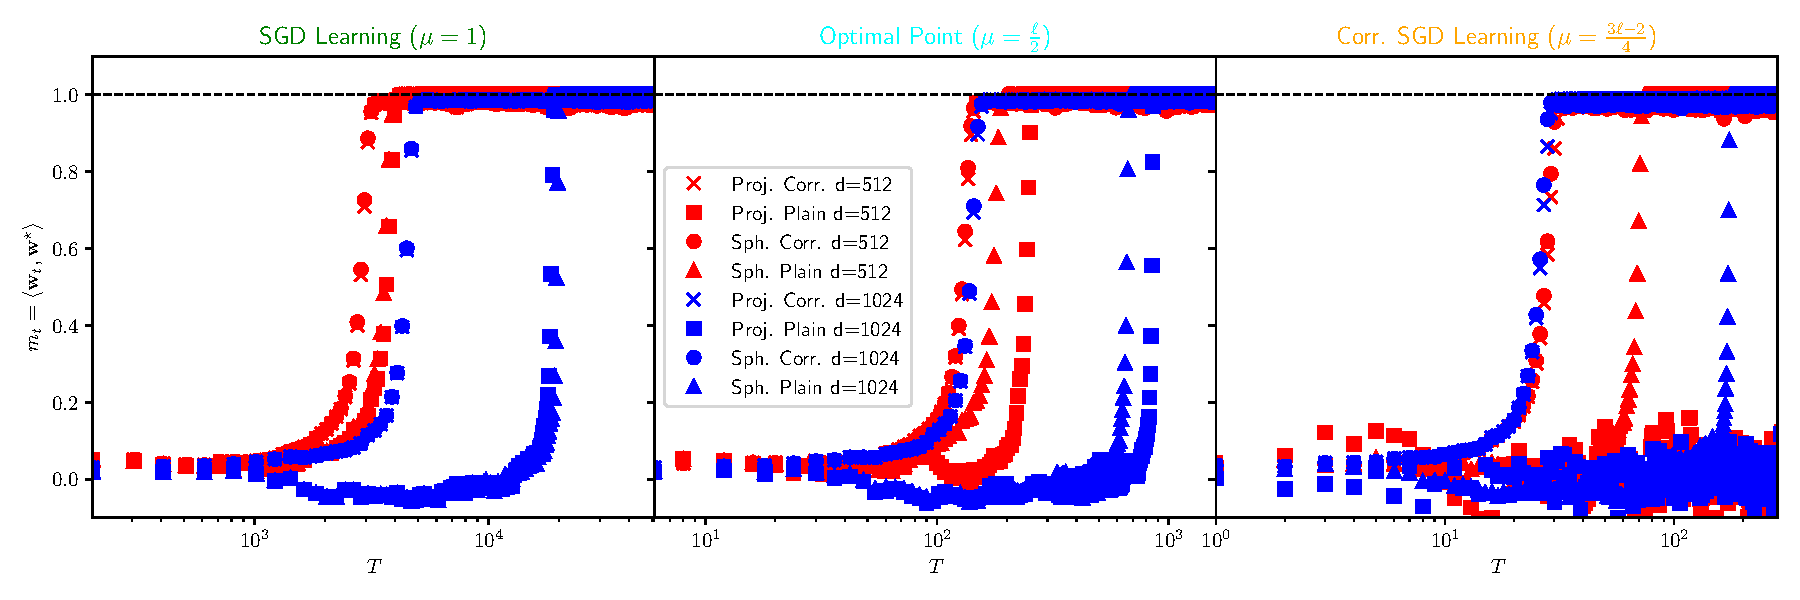
\includegraphics[width=\textwidth]{figs/H3H3_m_vs_T_spherical}
    \caption{\textbf{{Correlation Loss SGD} weak recovery:} Comparison between the performance of plain SGD, the Correlation Loss SGD and Spherical SGD, in different regions of the phase diagram, and for different sizes \(d\).
    The plot shows the test error as a function of the optimization steps. Both the teacher and the student activation functions are fixed to \(\sigma = h^\star =\text{He}_3\), so the information exponent is \(\ell=3\). In all the three plots we vary the value of \(\mu\), while \(\delta = \sfrac{\ell}{2} - \mu\).
    Spherical SGD learns even in regions forbidden for plain SGD, as the Correlation Loss does. Note that the Spherical Correlation Loss is equivalent to the Projected Correlation Loss in all the regimes.
    }
\label{2406:fig:app:spherical}
\end{figure}

\subsection{\emph{Adaptive SGD}: combining Correlation Loss SGD with plain SGD}

Despite these benefits, the correlation loss is not a good choice to fully learn the target. In this subsection, we explore the idea of combining the two algorithms to escape fast with correlation loss, and then reach the global minimum with the MSE loss.
We will call the combination of these two algorithms \emph{Adaptive SGD}.

We are going to test in the simplest case possible: GLM with \(\text{He}_3\) as activation function (we remark that there is no benefit in using Correlation Loss SGD over plain SGD when \(\ell\le2\)). If we run the algorithm for multi-index models, it would help to escape the initial saddle, but the algorithm may get stuck in another critical point that is not the global minimum. The study on how to escape fast from a critical point other than the initial one goes beyond the scope of this paper. Our \emph{Adaptive SGD} procedures works as follows:
\begin{enumerate}
    \item Make a Correlation Loss SGD step;
    \item If the Loss is smaller than 60\% of the initial loss, jump to Step~3, otherwise go back to Step~1;
    \item Reduce the learning rate of a factor \(0.995\) and do a Standard SGD step;
    \item If converged stop, otherwise go back to Step~3.
\end{enumerate}
The learning rate is progressively reduced because the plain SGD requires a lower learning rate compared to the one used by correlation loss to escape fast. Certainly, one can design a much more powerful algorithm than the one we present, but the goal here is just to show that the combination of the two is beneficial, and not to find the possible one.
\begin{figure}
    \centering
    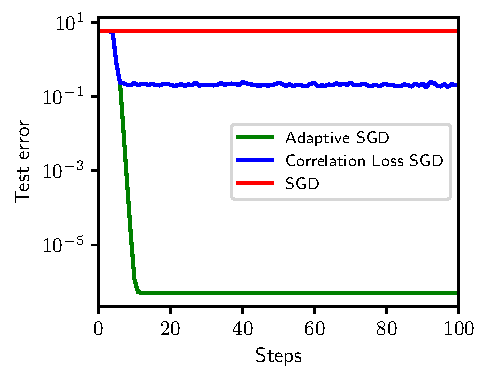
\includegraphics[height=0.49\textwidth]{figs/adaptive_SGD}
    \caption{\textbf{Adaptive SGD:} The plot compares the performance of SGD and Correlation loss SGD, algorithms with Adaptive SGD; this protocol consists of first using correlation loss SGD to achieve weak recovery, and then switch to adaptive SGD for learning the target. (\(\ell=3,\mu=1.85, \delta=\mu-\frac\ell2, \Delta=10^{-6}\)).}
    \label{2406:fig:app:adaptive}
\end{figure}
Figure~\ref{2406:fig:app:adaptive} shows how the Adaptive SGD Algorithm is the best one when fully learning the target.

\subsection{Polylog regime example} \label{2406:app:sec:polylog}
We showed in Section~\ref{2406:sec:main:cold_start} that it is possible to push down the number of steps needed to weakly recover the target until it is growing less than any power law. In order to achieve this, we need to run \emph{Correlation Loss SGD} with \(n_b > d^{\ell-1}\) and \(\gamma > O(d^{1-\sfrac\ell2})\), as pictured by Figure~\ref{2406:fig:app:deltamu_phasediagram}.
Proposition~\ref{2406:prop:main:exact_asympt} shows that our theory for cold start, based on expansion of the process \eqref{2406:eq:app:process}, is not valid, among other conditions, when \(\delta < 0\).
Therefore, the only case where we can simultaneously observe the \emph{polylog regime} and have an exact asymptotic description for the full dynamics is when \(\ell=2, \gamma = O(1)\) and \(n_b=O(d)\). Let's stick for simplicity with a GLM whose activation is \(\text{He}_2\). Note that the total sample complexity is always \(N = n_b T = O(d \log d)\).

\begin{figure}
    \centering
    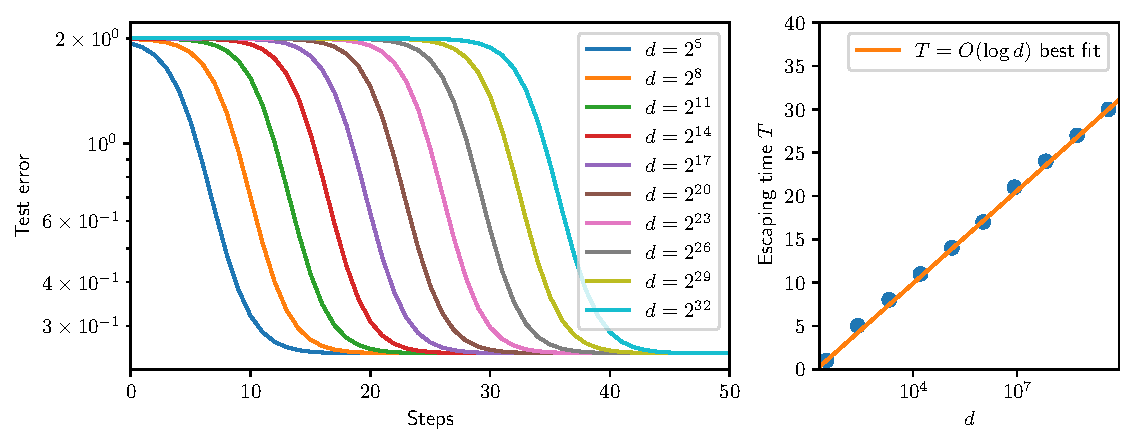
\includegraphics[width=\textwidth]{figs/polylog_region}
    \caption{\textbf{Phase retrieval with large batch size:} Numerical integration of the process \eqref{2406:eq:app:process}, for  \(f=f^\star=\text{He}_2, \gamma = O(1)\) and \(n_b=O(d)\). The escaping time dependence on the number of time steps is a \(T=O(\log d)\): we claim this to be valid for all the \emph{polylog regime}.}
    \label{2406:fig:app:subpower}
\end{figure}
Figure~\ref{2406:fig:app:subpower} shows a numerical test of our theory in this particular case. We see that as \(d\) grows, also the time needed to escape initial conditions grows. In the right part of the Figure we show that the exact dependence is \(T = O(\log d)\), that is indeed a polylog law.

\subsection{Large-batch corrections to asymptotic dynamics}
Although disappearing when taking the limit, the terms of evolution process \eqref{2406:eq:app:process} coming from intra-batch correlation are useful for providing a better description at large but finite \(d\). Effectively, they are behaving as a first correction to the asymptotic limit.

In this section, we aim to provide numerical arguments about the importance of intra-batch correlations at finite \(d\). We stick with the GLM setting, with \(\erf\) as activation function. Note that since the information exponent of this target is 1, there is no mediocrity at initialization, we can set \(m=\vec w^\top \vec w ^\star = 0\) without falling in the \emph{cold start regime}.
\begin{figure}
    \centering
    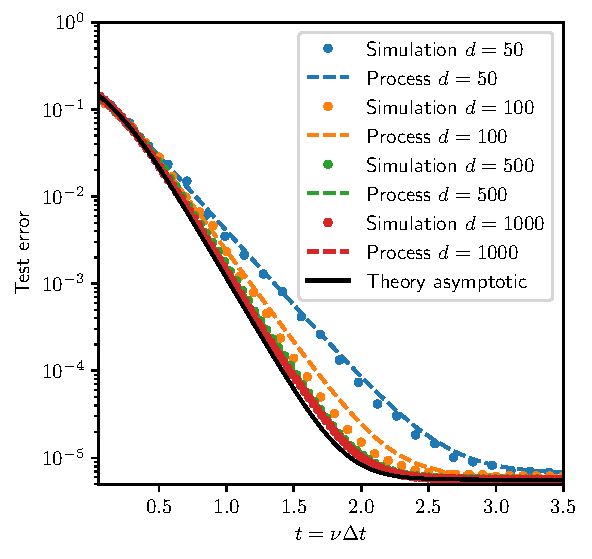
\includegraphics[height=0.3925\textwidth]{figs/finitesize_asymptotic_test_error}
    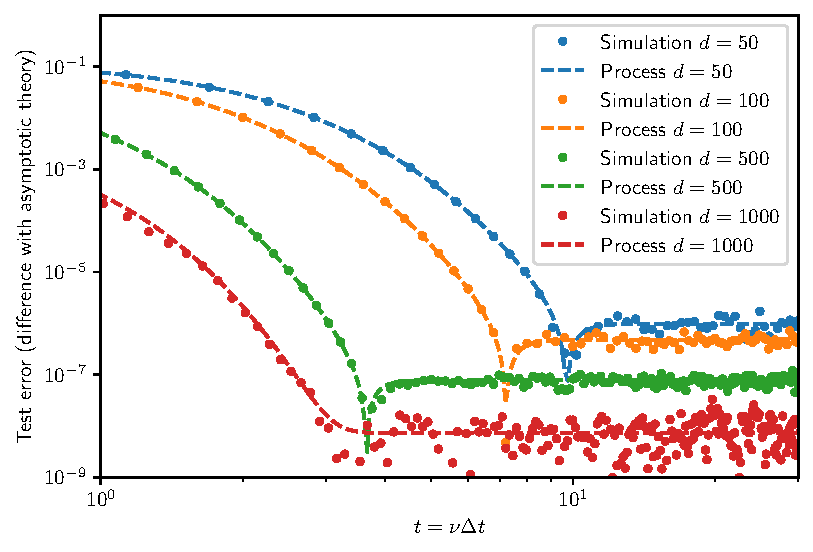
\includegraphics[height=0.3925\textwidth]{figs/finitesize_asymptotic_differnce}
    \caption{\textbf{Non asymptotic corrections:} Comparison between simulations (dots), exact asymptotic solution of ODE (continuous black line), and exact solution including the subleading large-batch corrections (dashed line). As expected, as \(d\to+\infty\) the simulations are getting closer and closer to the asymptotic solution; on the other hand, taking into account the batch correlations allows to have a better description of the dynamic even a small \(d\).}
    \label{2406:fig:app:finitesizeasym}
\end{figure}
Figure~\ref{2406:fig:app:finitesizeasym} shows simulations for different values of \(d\) (dots), accompanied by the full process dynamic that includes the intra-batch correlation terms (dashed lines); the asymptotic solution of the differential equations \eqref{2406:eq:spherical_closed_form_ode} is the continuous black line. To enlighten the process even more, we also shows the difference between the asymptotic solution, at the actual finite \(d\) one on the right part of the figure. We see that the full process solution always match with the actual project SGD simulation; most importantly, when \(d\) grows the simulations are getting closer and closer to the asymptotic solution, confirming that the large batch plays no effect in high-dimension.


% \input{sections/appendix/simple_explanation.tex}
